% Options for packages loaded elsewhere
\PassOptionsToPackage{unicode}{hyperref}
\PassOptionsToPackage{hyphens}{url}
\PassOptionsToPackage{dvipsnames,svgnames,x11names}{xcolor}
%
\documentclass[
  letterpaper,
  DIV=11,
  numbers=noendperiod]{scrartcl}

\usepackage{amsmath,amssymb}
\usepackage{iftex}
\ifPDFTeX
  \usepackage[T1]{fontenc}
  \usepackage[utf8]{inputenc}
  \usepackage{textcomp} % provide euro and other symbols
\else % if luatex or xetex
  \usepackage{unicode-math}
  \defaultfontfeatures{Scale=MatchLowercase}
  \defaultfontfeatures[\rmfamily]{Ligatures=TeX,Scale=1}
\fi
\usepackage{lmodern}
\ifPDFTeX\else  
    % xetex/luatex font selection
\fi
% Use upquote if available, for straight quotes in verbatim environments
\IfFileExists{upquote.sty}{\usepackage{upquote}}{}
\IfFileExists{microtype.sty}{% use microtype if available
  \usepackage[]{microtype}
  \UseMicrotypeSet[protrusion]{basicmath} % disable protrusion for tt fonts
}{}
\makeatletter
\@ifundefined{KOMAClassName}{% if non-KOMA class
  \IfFileExists{parskip.sty}{%
    \usepackage{parskip}
  }{% else
    \setlength{\parindent}{0pt}
    \setlength{\parskip}{6pt plus 2pt minus 1pt}}
}{% if KOMA class
  \KOMAoptions{parskip=half}}
\makeatother
\usepackage{xcolor}
\usepackage{soul}
\setlength{\emergencystretch}{3em} % prevent overfull lines
\setcounter{secnumdepth}{-\maxdimen} % remove section numbering
% Make \paragraph and \subparagraph free-standing
\ifx\paragraph\undefined\else
  \let\oldparagraph\paragraph
  \renewcommand{\paragraph}[1]{\oldparagraph{#1}\mbox{}}
\fi
\ifx\subparagraph\undefined\else
  \let\oldsubparagraph\subparagraph
  \renewcommand{\subparagraph}[1]{\oldsubparagraph{#1}\mbox{}}
\fi


\providecommand{\tightlist}{%
  \setlength{\itemsep}{0pt}\setlength{\parskip}{0pt}}\usepackage{longtable,booktabs,array}
\usepackage{calc} % for calculating minipage widths
% Correct order of tables after \paragraph or \subparagraph
\usepackage{etoolbox}
\makeatletter
\patchcmd\longtable{\par}{\if@noskipsec\mbox{}\fi\par}{}{}
\makeatother
% Allow footnotes in longtable head/foot
\IfFileExists{footnotehyper.sty}{\usepackage{footnotehyper}}{\usepackage{footnote}}
\makesavenoteenv{longtable}
\usepackage{graphicx}
\makeatletter
\def\maxwidth{\ifdim\Gin@nat@width>\linewidth\linewidth\else\Gin@nat@width\fi}
\def\maxheight{\ifdim\Gin@nat@height>\textheight\textheight\else\Gin@nat@height\fi}
\makeatother
% Scale images if necessary, so that they will not overflow the page
% margins by default, and it is still possible to overwrite the defaults
% using explicit options in \includegraphics[width, height, ...]{}
\setkeys{Gin}{width=\maxwidth,height=\maxheight,keepaspectratio}
% Set default figure placement to htbp
\makeatletter
\def\fps@figure{htbp}
\makeatother

\KOMAoption{captions}{tableheading}
\makeatletter
\makeatother
\makeatletter
\makeatother
\makeatletter
\@ifpackageloaded{caption}{}{\usepackage{caption}}
\AtBeginDocument{%
\ifdefined\contentsname
  \renewcommand*\contentsname{Table of contents}
\else
  \newcommand\contentsname{Table of contents}
\fi
\ifdefined\listfigurename
  \renewcommand*\listfigurename{List of Figures}
\else
  \newcommand\listfigurename{List of Figures}
\fi
\ifdefined\listtablename
  \renewcommand*\listtablename{List of Tables}
\else
  \newcommand\listtablename{List of Tables}
\fi
\ifdefined\figurename
  \renewcommand*\figurename{Figure}
\else
  \newcommand\figurename{Figure}
\fi
\ifdefined\tablename
  \renewcommand*\tablename{Table}
\else
  \newcommand\tablename{Table}
\fi
}
\@ifpackageloaded{float}{}{\usepackage{float}}
\floatstyle{ruled}
\@ifundefined{c@chapter}{\newfloat{codelisting}{h}{lop}}{\newfloat{codelisting}{h}{lop}[chapter]}
\floatname{codelisting}{Listing}
\newcommand*\listoflistings{\listof{codelisting}{List of Listings}}
\makeatother
\makeatletter
\@ifpackageloaded{caption}{}{\usepackage{caption}}
\@ifpackageloaded{subcaption}{}{\usepackage{subcaption}}
\makeatother
\makeatletter
\@ifpackageloaded{tcolorbox}{}{\usepackage[skins,breakable]{tcolorbox}}
\makeatother
\makeatletter
\@ifundefined{shadecolor}{\definecolor{shadecolor}{rgb}{.97, .97, .97}}
\makeatother
\makeatletter
\makeatother
\makeatletter
\makeatother
\ifLuaTeX
  \usepackage{selnolig}  % disable illegal ligatures
\fi
\IfFileExists{bookmark.sty}{\usepackage{bookmark}}{\usepackage{hyperref}}
\IfFileExists{xurl.sty}{\usepackage{xurl}}{} % add URL line breaks if available
\urlstyle{same} % disable monospaced font for URLs
\hypersetup{
  pdftitle={A LIMITED SCOPE OF THE COST OF AIR TRAVEL},
  pdfauthor={Adaeze Obinelo},
  colorlinks=true,
  linkcolor={blue},
  filecolor={Maroon},
  citecolor={Blue},
  urlcolor={Blue},
  pdfcreator={LaTeX via pandoc}}

\title{A LIMITED SCOPE OF THE COST OF AIR TRAVEL}
\author{Adaeze Obinelo}
\date{}

\begin{document}
\maketitle
\ifdefined\Shaded\renewenvironment{Shaded}{\begin{tcolorbox}[boxrule=0pt, interior hidden, breakable, frame hidden, sharp corners, enhanced, borderline west={3pt}{0pt}{shadecolor}]}{\end{tcolorbox}}\fi

\textbf{Full Title:} EVERYTHING IS AWFUL. OR IS IT? - A LIMITED SCOPE OF
THE COST OF AIR TRAVEL THROUGH THE YEARS (ONE THING THAT MAY NOT* BE
OBJECTIVELY AWFUL)

\textbf{Short Title:} LIMITED SCOPE ANALYSIS OF Q2 AIRFARE IN THE U.S.
OVER THE LAST 4 DECADES

\textbf{Author:} Adaeze Obinelo

\ul{\textbf{Introduction}}:

Today's political, economic, and social climate seems to be, on a good
day, a succession of inconveniences, and on the worst of days, a
never-ending cascade of unprecedented challenges and horrors. Especially
thanks to recent economic inflation, everyday necessities are taking a
greater and greater toll on the average consumer's wallet. Via the
consumer price index (CPI) (NBC news, 2023), the overall costs of food,
gas and shelter increased significantly over the summer. This increase
was certainly felt acutely here in Los Angeles, where gas rose as high
as \$6 in some areas, and food prices continued to climb. Purchasing my
airfare home this year, I felt the sting on my wallet particularly
severely, and I found myself wondering ``were airplane tickets always
this high?''. I am not inexperienced in air travel, having flown
frequently prior to college for athletics, during undergrad, and now as
an adult to visit family. For some reason, when I think back to
purchasing my tickets in the past, I cannot recall feeling the same
unenthusiastic and reluctant resignation that I felt this year. For this
reason, I thought it would be an interesting investigation to answer the
following question; ``How has airfare changes in the past few decades''.
The present report aims to do exactly this, using the United States
Bureau of Transportation Statistics (BTS) data on airfare.

\ul{\textbf{Methods}}:

The following analysis was conducted using the United States Bureau of
Transportation Statistic's (BTS) record of Average Domestic Itinerary
Fares. This dataset is compiled each financial quarter (Q1-Q4), and the
most recent financial quarter data available is from Q2 of 2023. For
each quarter, the dataset compiles average flight fares by airport by
year, year and these fares by a variable called ``2022 Passenger Rank'',
which is an ordinal variable calculated by comparing the value
equivalent to 10\% of all passengers served in 2022 (a variable also
included in each dataset).

Due to the data limitations for the current financial year, data from
the second financial quarter of 4 years, 1993, 2003, 2013, and 2023 was
utilized for analysis. A 10-year spread was thought to be ideal for
assessing the general trends in airfare data. The datasets from this
chosen time frames were downloaded directly from the Transportation
Bureau's website, using the above link, into .csv filed. Most of the
data processing and cleaning was done using the dplyr, tidyverse and
baseR packages. As part of data processing, variables names were altered
to aid in the coding process. Variable types were changed to the
appropriate type (continuous or character). Included in each dataset was
`2022 Passengers', a variable which compares the number of domestic
passengers each airport sees in 2022. A missing value or a value of 0
indicate these airports don't provide commercial domestic flights, so
entries with these values were removed since they would not be airports
the consumer is choosing from.

To additional analysis, coordinate data was taken from The Humanitarian
Data Exchange which compiled a dataset of longitude and latitude values
for 508 major US airports. This coordinate dataset was merged with the
BTS datasets. Cross-validation was done by comparing the inflation
adjusted fare variable for each year (Adjusted\_Avg\_Fare\_Q2) provided
originally with my dataset with an actual dollar to dollar conversion
between that year and 2023(Table 1: Results of cross-validation). A new
variable, ``check.adj.xx'' was created for each year of analysis by
multiplying the (Average\_xxxx) for each year by the inflation
adjustment to the 2023 dollar value (1993: 2.13, 2003: 1.67, 2013: 1.32,
2023: 1). States were categorized into ``East'' and ``West'' by U.S.
census geographic zones, with Northeast, south and Midwest considered
``East'' and all remaining states considered ``West''.

Given that the research question centers around LAX and BOS airports,
the overall dataset was queried for trends in relation to these two
airports. Due to the great geographic distance between these airports,
the overall dataset was stratified by location to better understand
region-specific baseline trends. Scatterplots were used to visualize
trends between continuous variables. Bar plots were used to visualize
continuous variables by geographic location.

\ul{\textbf{Results}}

The Passenger Rank of LAX and BOS remained constant across all four time
frames sampled; BOS ranking 6\textsuperscript{th}, and LAX ranking
1\textsuperscript{st} (Table 3), indicating that both airports see an
extremely high number of US domestic flights per time frame sampled.
However, neither LAX nor BOS were in states found to have the most
expensive airport to fly out of in any of the Q2 data sampled: The state
with the highest average adjusted airfare in 1993 was Georgia (477.24,
Table 1), the state with the highest average adjusted airfare in 2003
was New Mexico (531.44, Table 1), and the state with the highest
adjusted average airfare in 2013 and 2023 was Alaska (596.00 and 641.09,
Table 1). In comparison, the average airfare for California for 1993,
2003, 2013, and 2023 was 354.04, 342.62, 401.70 and 403.09, and the
average airfare in Massachusetts for the same timepoints was 305.94,
426.40, 363.57, 392.25. The most expensive airport to fly out of in 2023
was Cold Bay Airport in Alaska, and the least expensive to fly out of
was Santa Maria in California (Figure 4).

Comparing Passenger Rank to Inflation Adjusted Fare, it appears that as
passenger rank increases in the Western states, Inflation Adjusted
Average fare tended to increase for all time points (Figure 1). This
trend was largely mirrored in the Eastern U.S. States, for all years
except 1993, where there did not appear to be a strong association
between passenger rank and fare (Figure 2). Importantly, it appears that
adjusted airfare is lower in 2023 than it has been for the other time
points in both the east and the west. Comparing the dollar amount of the
average ticket at Logan and LAX between 1993 and 2023, one would be
paying around \$369 less for a ticket out of BOS, and around \$279 less
for a ticket out of LAX.

\ul{\textbf{Conclusion}}

~~~~~~~~~~~ Evidently, by inflation adjusted values, I am paying less
for a trip between LAX and BOS than I have in the past. This begs the
question of why it feels as if I am not. This can probably be answered
best by looking at the unadjusted fare comparisons in Figure 3. Looking
specifically at unadjusted fares out of Logan and LAX by year which show
that overall, the \emph{unadjusted} fare for airline tickets out of LAX
and BOS are higher in 2023 than compared to years prior. While inflation
adjusted values provide a good gauge of the ``true'' cost of a purchase
in relation to the strength of the dollar, unadjusted amounts are the
``ouch'' one feels when actually paying for something in the moment.
Since the unadjusted values are higher than they have been in the past,
this is likely why it anecdotally feels like airfare prices are going
up.

The above study does have significant limitations, namely that
limitations in man-power limit our analysis to 4 timepoints separated by
a decade. Due to this, this analysis definitely misses more acute
variation in the dataset, and additionally does not account for the
remaining financial quarters of the year.The above study does have
significant limitations, namely that limitations in man-power limit our
analysis to four time points separated by a decade. Due to this, this
analysis definitely misses more acute variation in the dataset, and
additionally does not account for the remaining financial quarters of
the year. However, limited though it may be, it does provide a bit of
assurance to those of us purchasing airfare.

Citations:

Jay, M. (2023, September 13). \emph{Inflation ticks upward to 3.7\% for
August 2023: Here's how it could affect interest rates}. NBCNews.com.
https://www.nbcnews.com/business/economy/inflation-august-2023-number-will-interest-rates-keep-going-up-rcna104655

\ul{\textbf{Figures and Tables:}}

\begin{figure}

{\centering 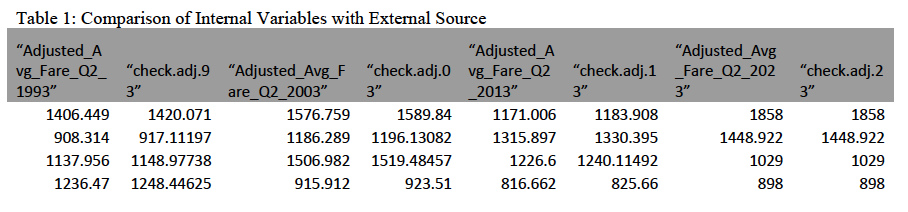
\includegraphics{images/Table1.png}

}

\end{figure}

\begin{figure}

{\centering 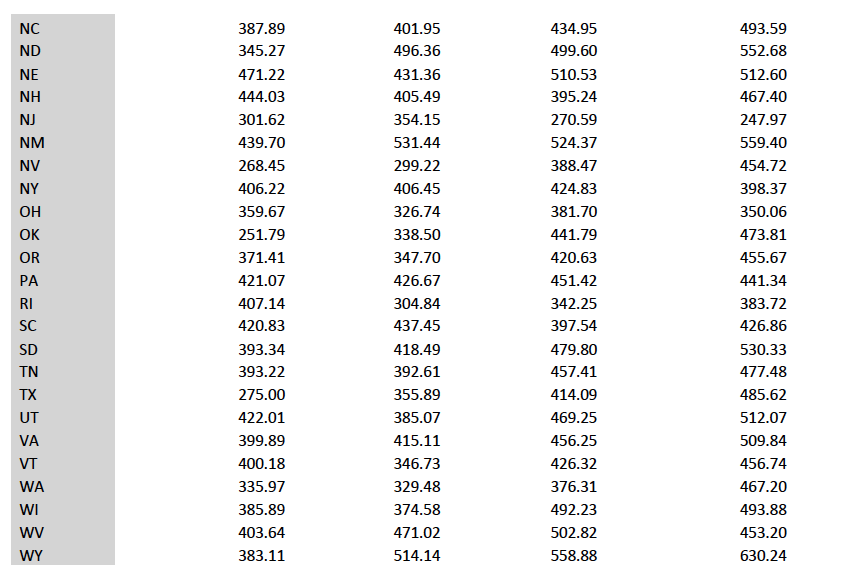
\includegraphics{images/Table2b.png}

}

\end{figure}

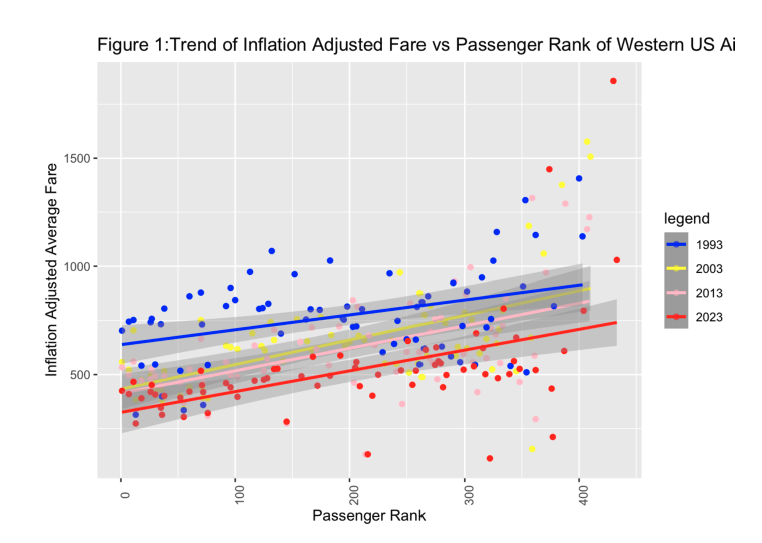
\includegraphics{images/Fig1-01.png}

\begin{figure}

{\centering 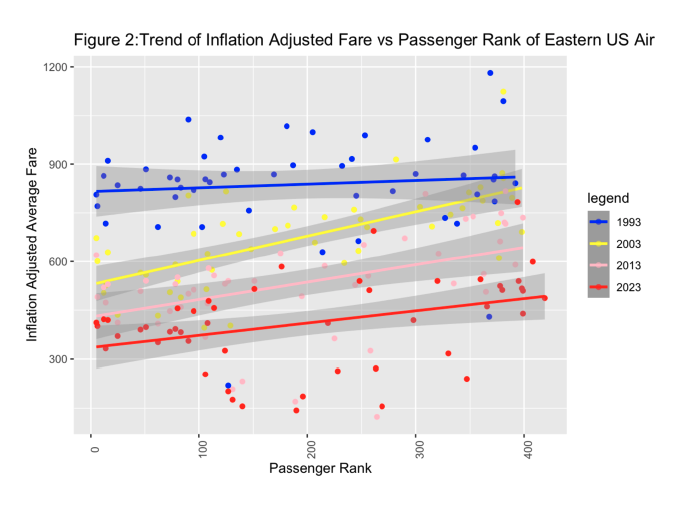
\includegraphics{images/Fig2-01.png}

}

\end{figure}

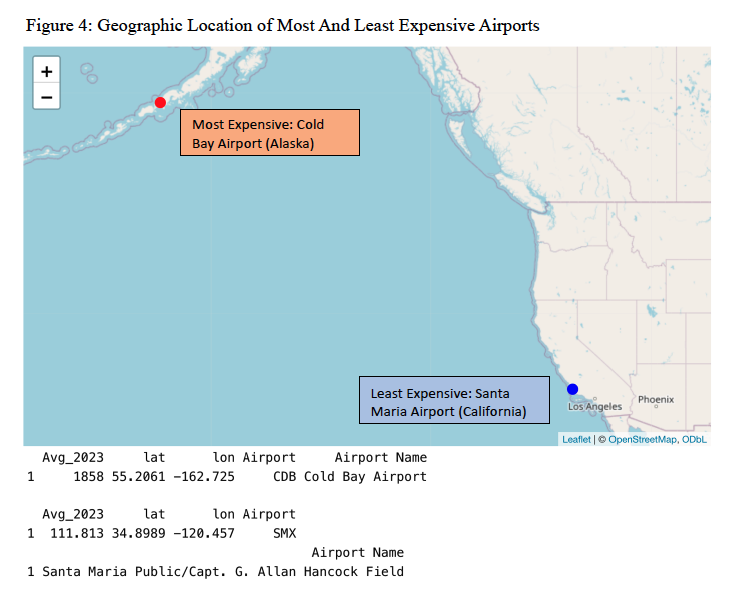
\includegraphics{images/Fig4-01.png}



\end{document}
